\documentclass{article}

% if you need to pass options to natbib, use, e.g.:
%     \PassOptionsToPackage{numbers, compress}{natbib}
% before loading neurips_2019

% ready for submission
% \usepackage{neurips_2019}

% to compile a preprint version, e.g., for submission to arXiv, add add the
% [preprint] option:
%     \usepackage[preprint]{neurips_2019}

% to compile a camera-ready version, add the [final] option, e.g.:
     \usepackage[final]{neurips_2019}

% to avoid loading the natbib package, add option nonatbib:
%     \usepackage[nonatbib]{neurips_2019}

\usepackage[utf8]{inputenc} % allow utf-8 input
\usepackage[T1]{fontenc}    % use 8-bit T1 fonts
\usepackage{hyperref}       % hyperlinks
\usepackage{url}            % simple URL typesetting
\usepackage{booktabs}       % professional-quality tables
\usepackage{amsfonts}       % blackboard math symbols
\usepackage{nicefrac}       % compact symbols for 1/2, etc.
\usepackage{microtype}      % microtypography
\usepackage{graphicx}
\usepackage{subfig}

\title{Implementing GAN on MNIST and SVHN}

% The \author macro works with any number of authors. There are two commands
% used to separate the names and addresses of multiple authors: \And and \AND.
%
% Using \And between authors leaves it to LaTeX to determine where to break the
% lines. Using \AND forces a line break at that point. So, if LaTeX puts 3 of 4
% authors names on the first line, and the last on the second line, try using
% \AND instead of \And before the third author name.

\author{%
  Shengjie Sun \\
  ss5593\\
  Department of Statistics\\
  Columbia University\\
  New York, NY 10027 \\
  \texttt{ss5593@columbia.edu} \\
  % examples of more authors
  \And
  Zeyu Yang \\
  zy2327 \\
  Department of Statistics\\
  Columbia University\\
  New York, NY 10027 \\
  \texttt{zy2327@columbia.edu}
  % \AND
  % Coauthor \\
  % Affiliation \\
  % Address \\
  % \texttt{email} \\
  % \And
  % Coauthor \\
  % Affiliation \\
  % Address \\
  % \texttt{email} \\
  % \And
  % Coauthor \\
  % Affiliation \\
  % Address \\
  % \texttt{email} \\
}

\begin{document}

\maketitle

\begin{abstract}
  We implement DCGAN on MNIST and SVHN dataset.
  The generated samples for both datasets are great although it takes quite some time to train the model.
  To help the model converge faster, we implement WGAN as well.
  The result \textbf{TBD}.
\end{abstract}

\section{Introduction}

Generative Adversarial Nets (GAN), first introduced by Ian Goodfellow in 2014[1], is a model that can be used to generate new images. 
It has been a hot topic since then.

The core idea of GAN is to create a two-player game. 
Build a generator that creates fake images while the discriminator tells whether the image is true or fake.

We train $D$ to maximize the probability of assigning the
correct label to both training examples and samples from G. 
We simultaneously train G to minimize $log(1-D(G(z)))$.

The optimum case is that the generate can fully recover the distribution of the data and the discriminator cannot tell whether the image is fake or not i.e. the output of discriminator is $1/2$.

\section{Implmentation on MNIST}

\subsection{Architecture}

We used Deep Convoltional GAN (DCGAN)[2] as our structure.

\subsubsection{Generator}

\begin{itemize}
  \item First layer: Dense
    \begin{itemize}
      \item Input: $100 \times 1$ vector
      \item Output $7\times 7\times 256$
      \item Batch normalization
      \item Activation: leaky relu
    \end{itemize}
  \item Second layer: Conv2DTranspose
    \begin{itemize}
      \item Filter: 128
      \item Kernel size: 5
      \item Stride: 1
      \item Padding: same
      \item Batch normalization
      \item Activation: leaky relu
  \end{itemize} 
  \item Third layer: Conv2DTranspose
    \begin{itemize}
      \item Filter: 64
      \item Kernel size: 5
      \item Stride: 2
      \item Padding: same
      \item Batch normalization
      \item Activation: leaky relu
    \end{itemize}   
  \item Fourth layer: Conv2DTranspose
    \begin{itemize}
      \item Filter: 1
      \item Kernel size: 5
      \item Stride: 2
      \item Padding: same
      \item Activation: tanh
    \end{itemize}   
\end{itemize}

\subsubsection{Discriminator}

\begin{itemize}
  \item First layer: Conv2D
    \begin{itemize}
      \item Input: $28 \times 28\times 1$ array
      \item Filter: 64
      \item Kernel size: 5
      \item Stride: 2
      \item Padding: same
      \item Activation: leaky relu
      \item Dropout: 0.3
  \end{itemize} 
  \item Third layer: Conv2D
    \begin{itemize}
      \item Filter: 128
      \item Kernel size: 5
      \item Stride: 2
      \item Padding: same
      \item Activation: leaky relu
      \item Dropout: 0.3
    \end{itemize}   
  \item Fourth layer: Conv2D
    \begin{itemize}
      \item Filter: 256
      \item Kernel size: 5
      \item Stride: 2
      \item Padding: same
      \item Activation: leaky relu
      \item Dropout: 0.3
    \end{itemize} 
  \item Fifth layer: Flatten
  \item Sixth layer: Dense with output 1
\end{itemize}

\subsubsection{Hyperparameters}

\begin{itemize}
  \item Epoch: 
  \item Batch: 
  \item Learning rate
    \begin{itemize}
      \item Generator: 1e-3
      \item Discriminator: 1e-4
    \end{itemize}
\end{itemize}

\subsection{Result}

Training process in tensorboard



the generated samples compared with training dataset and figure 2a in paper

\begin{figure}[!htb]
  \centering
  \subfloat[MNIST data]{
  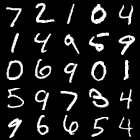
\includegraphics[width=0.2\textwidth]{mnist_data.png}}
  \subfloat[Epoch 10/50]{
  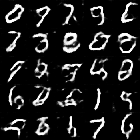
\includegraphics[width=0.2\textwidth]{I1.png}}
  \subfloat[Epoch 30/50]{
  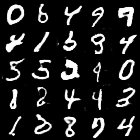
\includegraphics[width=0.2\textwidth]{I2.png}}
  \subfloat[Epoch 50/50]{
  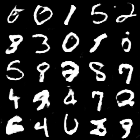
\includegraphics[width=0.2\textwidth]{I3.png}}
  \caption{Comparison of MNIST data and generated samples from DCGAN}
  \label{fig:DCGAN_MNIST}
\end{figure}

From Figure ~\ref{fig:DCGAN_MNIST}, 
we can see the generated samples has a good approximation after 30 epoches.

The samples from 10th are quite blury and they cannot have a good representation of number 2, 5, 8, etc.

The latter samples are clearer and the edges of the numbers are smoother. Number 0, 1, 3, 5, 7, 9 are quite ideal.

\section{Implmentation on SVHN}

\subsection{Architecture}

\subsubsection{Generator}

The generator is slightly modifed from the generator for MNIST. 
The output of the first dense layer is changed to $8\times 8\times 256$ 
and the filter of the fourth layer (Conv2DTranspose) has changed from 1 to 3
so that the output of the whole generator would be a $32\times 32\times 3$ image.

\subsubsection{Discriminator}

Discriminator is exactly the same as the previous one.

\subsection{Result}

Training process in tensorboard

the generated samples compared with training dataset

\begin{figure}[!htb]
  \centering
  \subfloat[SVHN data]{
  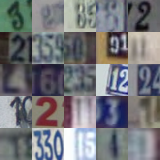
\includegraphics[width=0.2\textwidth]{svhn_data.png}}
  \subfloat[Epoch 10/50]{
  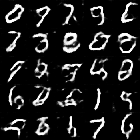
\includegraphics[width=0.2\textwidth]{I1.png}}
  \subfloat[Epoch 30/50]{
  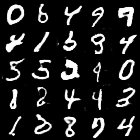
\includegraphics[width=0.2\textwidth]{I2.png}}
  \subfloat[Epoch 50/50]{
  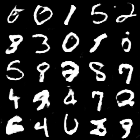
\includegraphics[width=0.2\textwidth]{I3.png}}
  \caption{Comparison of MNIST data and generated samples from DCGAN}
  \label{fig:DCGAN_SVHN}
\end{figure}

How is the quality compared to your GAN on MNIST? If the training does not go well, what failure modes do you see?

\section{WGAN}

Wasserstein GAN is a modified GAN introduced by Arjovsky, Martin, et al.(2017)[3]. 
It proposed Wasserstein that has a better property than Jensen-Shannon divergence.

\subsection{WGAN on MNIST}

xxx

\subsection{WGAN on SVHN}

xxx

\section{Summary}

xxx

\subsection{Future steps}

Self-attention neural network.

\section*{References}

[1] Goodfellow, Ian, et al. "Generative adversarial nets." Advances in neural information processing systems. 2014.

[2] Radford, Alec, Luke Metz, and Soumith Chintala. "Unsupervised representation learning with deep convolutional generative adversarial networks." arXiv preprint arXiv:1511.06434 (2015).

[3] Arjovsky, Martin, Soumith Chintala, and Léon Bottou. "Wasserstein gan." arXiv preprint arXiv:1701.07875 (2017).

\end{document}
